\subsection{Shadowing}
\label{sec:shadowing}
Roof surfaces may be shadowed by several object, such as other buildings, trees or even equipment on the roof itself. Since, the data source is a LOD 2 model only other buildings can be considered, because trees and roof equipment are not part of the model. The consideration of the shadowing may be done with a complicated illumination computation. Since this project is limited in time this is not possible. Therefore only a simple approach is applied, which completely ignore buildings which are shadowed, rather then adjusting the daily global irradiance on the specific surface.
Within the simple approach a building is neglected, if there is a neighboured building which is $x$ higher and is within a certain radius $r$. Only buildings between an azimuth of 90° to 270° are taken into account, as shown in Figure \ref{fig:shadow}.

\begin{figure}[ht]
	\centering
	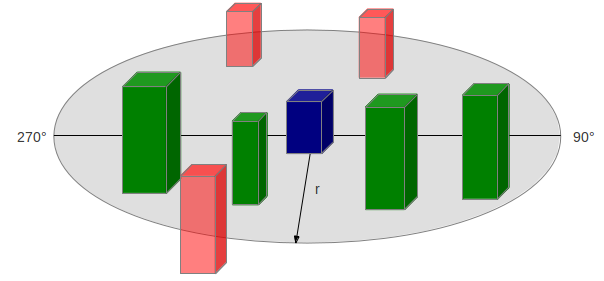
\includegraphics[width=0.7\textwidth]{phase2/group2/figure/fig_shadow.png}
	\caption{The green buildings are candidates, which may shadow the blue building}
	\label{fig:shadow}
\end{figure}

The implemented algorithm starts with iterating over all buildings and storing them in a spatial tree to make them easy queryable. After that before a potential of a building is calculated it will be checked if there are candidate buildings which are within the radius $r$. The list of candidates is checked for buildings which also meet the other conditions, such as an azimuth between $90^\circ$ and $270^\circ$ and if the building is $x$ times higher. If both conditions are met, the building will be neglected for the potential calculation. 